\documentclass{article}
\usepackage{tikz}
\begin{document}
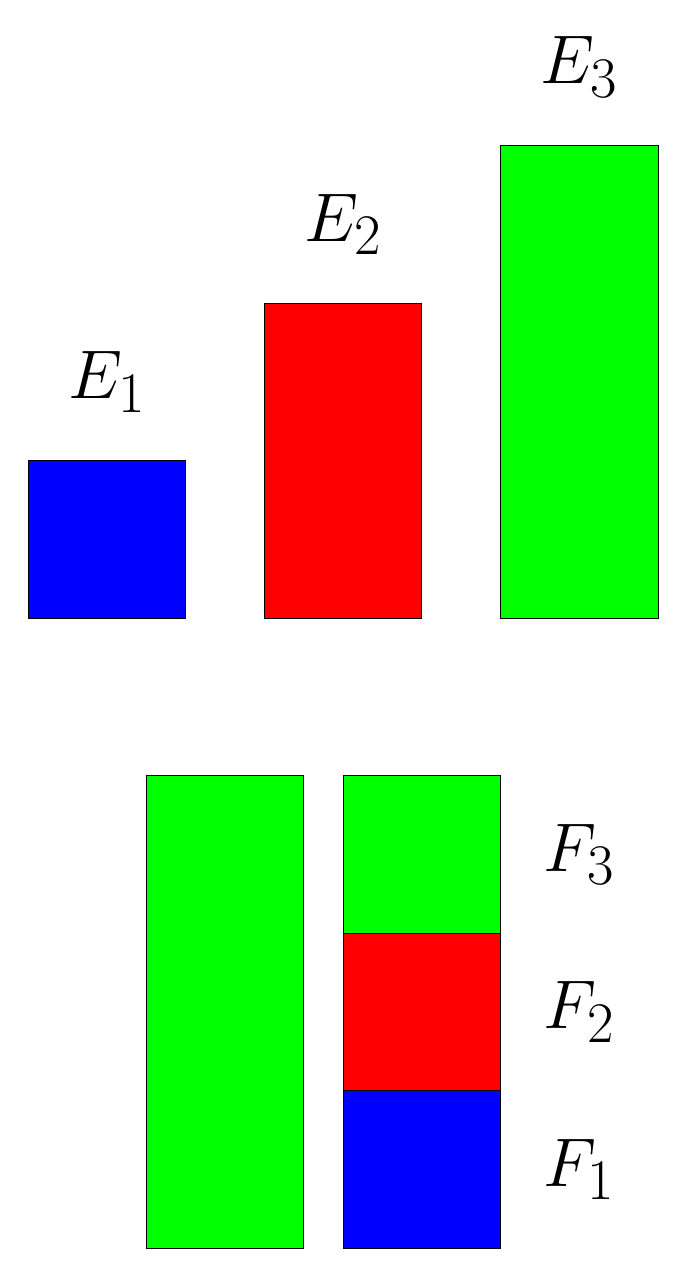
\begin{tikzpicture}
    \begin{scope}
	\draw[fill=blue] (0,0) rectangle (2,2);
	\node at (1,3) {\Huge$E_1$};
    \end{scope}
    \begin{scope}[xshift=3cm]
	\draw[fill=red] (0,0) rectangle (2,4);
	\node at (1,5) {\Huge$E_2$};
    \end{scope}
    \begin{scope}[xshift=6cm]
	\draw[fill=green] (0,0) rectangle (2,6);
	\node at (1,7) {\Huge$E_3$};
    \end{scope}
    \begin{scope}[xshift=1.5cm,yshift=-8cm]
	\draw[fill=green] (0,0) rectangle (2,6);
	%\node at (-3.0,-3) {\Huge$E_1{\cup}E_2{\cup}E_3 = E_3$};
    \end{scope}
    \begin{scope}[xshift=4cm,yshift=-8cm]
	\draw[fill=blue] (0,0) rectangle (2,2);
	\draw[fill=red] (0,2) rectangle (2,4);
	\draw[fill=green] (0,4) rectangle (2,6);
	\node at (3,1) {\Huge$F_1$};
	\node at (3,3) {\Huge$F_2$};
	\node at (3,5) {\Huge$F_3$};
    \end{scope}
\end{tikzpicture}
\end{document}
